%\todo{Make sure that all $k$-space functions have tildes.  Or not, but be consisitent with other chapters.}
\begin{figure}[ht]
 \centering
 \import{includes/}{setpgfinc}
 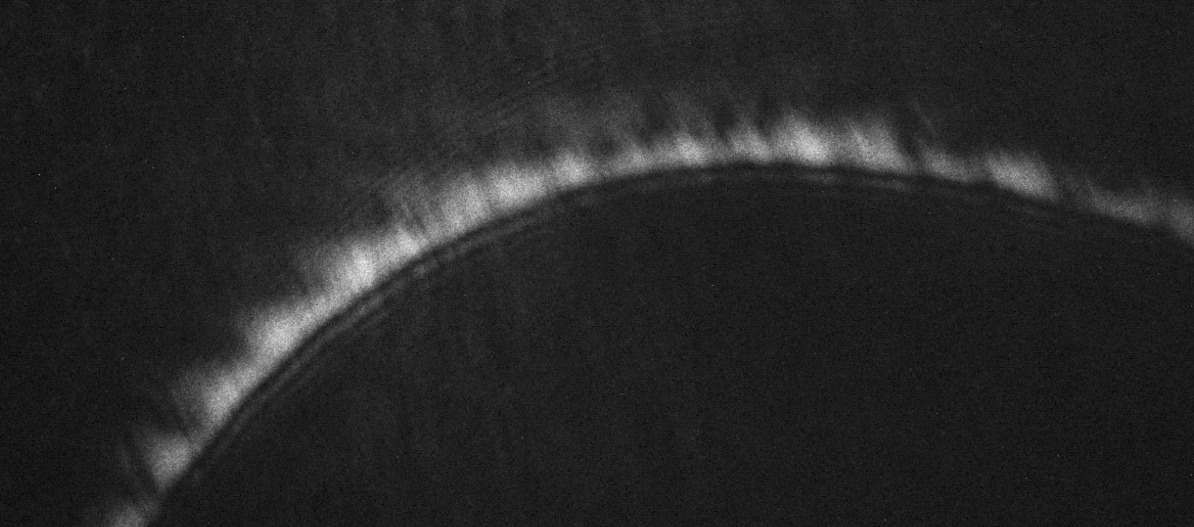
\includegraphics[keepaspectratio,width=0.9\textwidth]{interference/figures/coneintro.png}
 \caption{Section of the cone exhibiting one sided interference fringes.
 System parameters: $\lambda_0 = \SI{632.8}{\nano\meter}$,
 $n_1=1.9961$ (LAH79), $n_2 = \num{-14.4824 + 1.0946i}$ (Ag), $n_3=1.0$
 (air), and $d_2=\SI{48}{\nano\meter}$.}
\label{fig:coneintrofig} 
\end{figure}

When SPPs are excited in a prism coupled setup using a focused beam, it is
possible to observe a a curious one-sided oscillation pattern in either the
specular or conically scattered light~\cite{webster2013interference}.
Surprisingly, despite the popularity of SPR as a biosensing tool this
phenomena went unreported until
2005~\cite{schumann2008near}~\cite{andaloro2005optical}, and has since then
only been reported in a handful of limited
cases~\cite{shan2009measuring}~\cite{simon2007observation}.  An example of
this pattern is shown in \Figure{fig:coneintrofig} for a silver film on
high refractive index (LAH79) glass in air.

There are a number of reasons why these guys are important.  First, the
description of them being whatever interference between specularly
reflected beam is wrong.  And second, they may provide additional features
with which to increase fitting accuracy or whatever.

This chapter is something devoted to the study of these guys.

\section{Theory}
For simplicity we restrict the problem to the $x$-$z$ plane.  Consider an
incident $p$-polarized Gaussian beam passing through a prism evanescently
exciting either normal or long range SPPs on a metal film.  On the film,
the Gaussian beam may be represented in $k$-space as $\tilde{g}(k_x)$,
where
\begin{align}
\tilde{g}(k_x) &= \frac{w_0}{\sqrt{2}} \exp\left(\frac{1}{4}w_0\left(k_x - \ksp\right)\right)\\
&= \intinfty g(x)\, \me^{\mi k_x x} \md x
\end{align}
and
\begin{equation}
g(x) = \exp\left(-\frac{x^2}{w_0^2} + \mi \ksp x\right)
\end{equation}
where $w_0$ denotes the Gaussian beam waist parameter at the focus.  In the
specular direction, the field $\tilde{E}_\mathrm{notch}(k_x)$ is given by its
Fresnel reflectivity $\tilde{r}(k_x)$ multiplied by $\tilde{g}(k_x)$
\begin{equation}
\tilde{E}_\mathrm{notch}(k_x)=\tilde{g}(k_x)\,\tilde{r}(k_x)
\end{equation}
We assume $p$ polarization for the rest of this chapter and omit the
superscripts.

Let us now consider the spatial evolution of the light as it propagates
away from the surface.
The complete field in both $x$ and $z$ can be obtained by computing
the Fourier transform of $\tilde{E}_\mathrm{notch}(k_x)$ multiplied 
by a free space transfer function $\me^{\mi k_{z} z}$
\begin{align}
E_\mathrm{notch}(x,z) &= \intinfty \tilde{E}_\mathrm{notch}\, \me^{\mi k_{z,1} z}\, \me^{\mi k_x x} \md k_x\\
 &= \intinfty \tilde{g}(k_x)\, \tilde{r}(k_x)\, \me^{\mi \sqrt{k_0^2 \epsilon_1 - k_x^2}z}\, \me^{\mi k_x x} \md k_x
\label{eqn:fourier123}
\end{align}
Likewise, conically scattered light may be found using the same treatment
\begin{align}
E_\text{cone}(x,z) = \intinfty \tilde{g}(k_x)\, 
\tilde{t}_+(k_x)\, \tilde{t}_-(k_x)\,\me^{\mi k_z z}\, \me^{\mi k_x x} \md k_x
\label{eqn:fourier321}
\end{align}
Though this integral seems to have no analytic solution, its evaluation is
nonetheless straightforward on a computer.

\section{Experiment}
\begin{figure}[ht]
 \centering
 \import{includes/}{setpgfinc}
 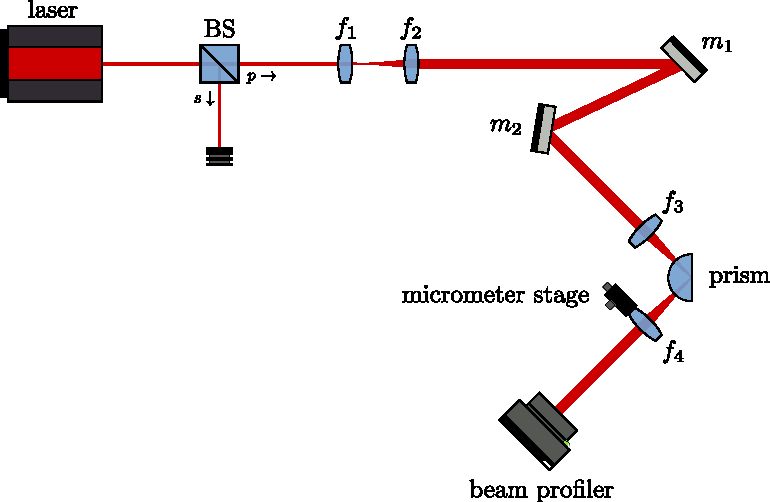
\includegraphics[keepaspectratio,width=10cm]{interference/figures/opticalsetup.pdf}
 \caption{Experimental setup used in this section.  Laser light passes
 through BS passing p-polarized light which is expanded by $f_1$ and $f_2$.
 $m_1$ and $m_2$ steer the expanded beam to $f_3$ which focuses it to the
 hypotenuse of the hemispherical prism.  $f_4$ re-images the reflected
 field to a beam profiler where it is recorded.}
 \label{fig:opticalsetup}
\end{figure}
Experimental verification of the predictions of \Equation{eqn:fourier123}
and \Equation{eqn:fourier321} was performed with the setup shown in
\Figure{fig:opticalsetup}.  Light from a
randomly polarized \SI{30}{\milli\watt} \SI{632.8}{\nano\meter} helium-neon
laser first passes through the polarizing
beamsplitter BS.  It is then expanded and re-collimated by $f_1$ and $f_2$ as an
approximately Gaussian beam with a $1/\me^2$ beam waist of
\SI{3}{\milli\meter} The light is steered by $m_1$ and $m_2$ to $f_3$, a
$f=\SI{20}{\milli\meter}$ antireflection coated aspherical lens, which
focuses the light to the central point of the hypotenuse of a
\SI{10}{\milli\meter} diameter LAH79 hemispherical prism
($n(\SI{632.8}{\nano\meter})\approx1.98$).  The beam makes a central angle
of $\theta_\text{sp}\approx\SI{32}{\degree}$ with the hypotenuse.
On the hypotenuse of the prism is a \SI{49.8}{\nano\meter} silver film
obtained through a sputtering process.  This thickness was chosen because
it optimizes the far field ATR minimum in the specularly reflected
direction.  Silver was used because it has the longest SPP propagation
length of all readily available sputtering targets.
Consistent with the Fourier optics perspective, a longer SPP propagation
length on the interface results in a narrower resonance linewidth in the
far field and vice versa.  A LAH79 hemispherical prism was used because of
its high refractive index ($n\approx 1.98$ at \SI{632.8}{\nano\meter}) and
because its hemispherical shape permits observation of scattered light with
minor distortion.  The totally internally reflected or scattered light is
optionally imaged at this point by the lens $f_4$, which is identical to
$f_3$.  The optical fields are observed by direct projection on a 10-bit
CCD sensor (beam profiler).  Since most of the interesting spatial structure of the
reflected beam occurs in a small spatial range, $f_4$
is mounted on a micrometer stage.  As the stage is translated, different focal
planes can be imaged.

\begin{figure}[ht]
 \centering
 \import{includes/}{setpgfinc}
	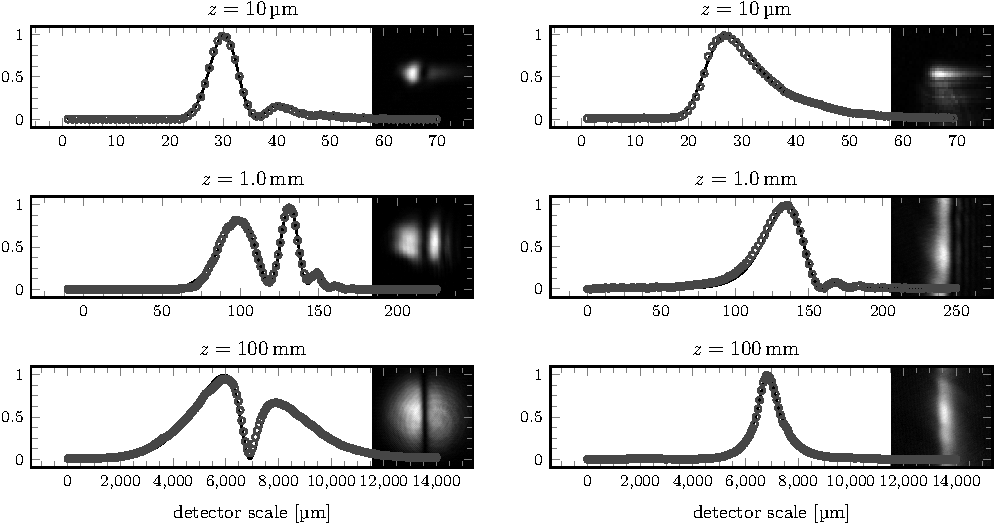
\includegraphics{interference/figures/fig2-crop.pdf}
	\caption{ Theoretical and experimental values of
$|E_\text{notch}(x,z)|^2$ and $|E_\text{cone}(x,z)|^2$ obtained for three
characteristic propagation distances.  Theoretical values are solid lines,
while experimental values are shown with points.  Distances are
approximate.  Inset is the experimentally obtained optical intensity.}
 \label{fig:fresnelprop}
\end{figure}
Verification of the optical fields were obtained using a beam profiler for
an optimally focused $f_3$ while the focal plane of $f_4$ was moved normal
to the direction of radiation.  Images at increasing distances from the
surface were taken or light in both the notch
($\phi=0$) and the cone at an angle $\phi = \SI{90}{\degree}$.  Since the
cone is more or less radially isotropic, the choice of $\phi$ in this
experiment is arbitrary as long as it is far enough away from the incident
or specular beam.  This data is shown in \Figure{fig:fresnelprop}.  Here is
shown theoretical calculations based on \Equation{eqn:fourier123} and
\Equation{eqn:fourier321} alongside linear (2D) sections of the experimentally obtained results for
three different characteristic propagation distances.  The first and last
are representative of the near and far field, and their optical fields are
related by a simple Fourier transform pair.  The middle propagation
distance was chosen because of the high visibility of the oscillations in
this region.  As is evident from the figures, as the field propagates it
diffracts, and between the near and far fields a one-sided oscillatory
structure occurs.  The experimentally obtained field matches well with
theoretical calculations using an unmodified Drude model for Ag.

At $z=0$, $|E_\text{notch}(x,z=0)|^2$ matches surface field theoretically
predicted via a similar method by~\cite{chuang1986lateral}, or through
vector Gaussian beam decomposition~\cite{baida1999theoretical}.  This has
also been experimentally verified through near field optical measurements
(SNOM), though this only permits observation of the field on the 2-3
interface, or $|E_\text{cone}(x,z=0)|^2$.  Near field measurements of the
1-2 interface are not possible due to the presence of the prism.  It is
interesting that we have obtained both fields using optical-only methods;
here both SPP propagation and radiative decay are observed simultaneously.

The far field is often defined as as $z\gg 2 D^2/\lambda$, where $D$ is the
spatial width of the source.  For Ag at \SI{632.8}{\nano\meter}, the Drude
model permittivity is $\epsilon \approx \num{-16.858+0.437i}$ and the
$1/\me$ SPP propagation distance normal to the interface $D = 1/(2 k_x)
\approx \SI{60}{\micro\meter}$ and the resulting far field limit is $2
D^2/\lambda \approx \SI{10}{\milli\meter}$.  This seems to be consistent
with both the simulated and experimental results, as it is approximately
the distance in \Figure{fig:fresnelpropagate} for which the oscillations
disappear.

\subsection{Interference and Diffraction}
Previous reports of the oscillations in the specular direction for long
range surface plasmons~\cite{simon2007observation} and localized surface
plasmons~\cite{schumann2008near} have described it as arising due to
interference between the specular reflection of the Gaussian beam from the
1-2 interface and the re-radiated plasmon field from the 2-3 interface.
These components can be identified by the two peaks in
$|E_\text{spec}(x,z=0)|^2$.  While it is true that the field in the
specular direction contains both components, and that $\tilde{r}_{12}$ and
$\tilde{r}_{23}$ are indeed antiphase at $k_\text{sp}$ the one-sided
oscillatory pattern does not require a specular component to be observed.
This is evidenced in several ways.
\begin{figure}[ht]
 \centering
 \import{includes/}{setpgfinc}
 \import{interference/figures/}{r123m12}
 %\includegraphics[keepaspectratio,width=10cm]{<++>}
\caption{Comparison of the propagated $\tilde{r}_{123}(k_x)$ verses
$(\tilde{r}_{123}(k_x)-\tilde{r}_{12})$.  Note that oscillations occur in
both cases.  }
 \label{fig:r123m12}
\end{figure}

First, we can mathematically remove the contribution of the 1-2 interface
by propagating $\tilde{r}_{123}-\tilde{r}_{12}$.  This has been done in
\Figure{fig:r123m12} for $z=\SI{1.17}{\milli\meter}$.  Note that the
oscillations persist, despite the absence of $\tilde{r}_{12}$.  In terms of
the experiment this is equivalent to the profile found in the conically
scattered light, itself containing spatial oscillations.

In light of these observations, it is more correct to ascribe the one-sided
oscillatory structure as being a diffraction, rather than a two component
interference phenomena motivated by phase alone.  In passing we note that this can also be found in
almost any causal function propagated by a free space transfer
term. As a paragon example, the Fourier transformed Lorentzian
absorption $\tilde{f}(k) = 1/(1+\mi k)$ qualitatively displays the
phenomena of the conical radiation when propagated.

\subsection{Evanescent Solutions}
In the context of diffraction integrals, the free space transfer function
$\exp(\mi k_{z,1} z)$ is often concerned with evanescent and propagating
terms, giving rise to the diffraction limit.  Here,
$k_{z,1}=\sqrt{k_0^2 \epsilon_1 - k_x^2}$ is imaginary for $k_0^2
\epsilon_1 < k_x^2$.  It is interesting to note that this never occurs.
Ignoring the condition for total internal reflection, 
$k_x = k_0 \sqrt{\epsilon_1} \sin \theta$ and we can set up an inequality
\begin{align}
k_0^2 \epsilon_1 &< k_x^2\\
k_0^2 \epsilon_1 &< \left(k_0 \sqrt{\epsilon_1} \sin \theta\right)^2\\
k_0^2 \epsilon_1 &< k_0^2 \epsilon_1 \sin^2 \theta\\
1 &< \sin^2 \theta
\end{align}
which is false, suggesting that if all light is collected, no information is
lost during propagation from the near to far field.
\section{The Fourier Optics Perspective}
There are several perspectives of SPR phenomena which can be insightful in
explaining why exactly the spatial oscillations are one-sided.  The first
is an argument from causality.  Assume a complex function $\chi(\omega) =
\chi'(\omega) + \mi \chi''(\omega)$ whose real and imaginary parts are
related by Kramers-Kronig relations
\begin{align}
\chi(\omega)=\mi \hf{\chi(\omega)}
\end{align}
with 
\begin{align}
\chi'(\omega) &= \hf{\chi''(\omega)}\\
\chi''(\omega) &= -\hf{\chi'(\omega)}
\end{align}
where $\hf{\chi(\omega)}$ is the Hilbert transform of $\chi(\omega)$.
The Fourier transform of $\chi(\omega)$ is
\begin{align}
\chi(\omega) &= \chi'(\omega) + \mi \chi''(\omega)\\
\ff{\chi(\omega)} &= \ff{\chi'(\omega) + \mi \chi''(\omega)}\\
&= \ff{\chi'(\omega)} + \ff{\mi \chi''(\omega)}\\
&= \ff{\chi'(\omega)} + \ff{\mi \hf{\chi'(\omega)}} \\
&= \ff{\chi'(\omega)} + \sgn(\omega) \ff{\chi'(\omega)} \\
\end{align}
Or succinctly,
\begin{align}
\ff{\hf{\chi(\omega)}} = (-\mi \sgn(\omega)) \ff{\chi(\omega)}
\end{align}
In other words, the Fourier transform of any function which satisfies
Kramers-Kronig relations is ``one-sided'' as a necessary
condition of causality.  This seems to be true for the Fresnel
reflectivity as well as the complex permittivity.

The second perspective is couched in Fourier optics.  Here, because
SPR occurs at the focus of a Gaussian beam, it can be seen as a sort of
spatial filter which modifies the local $k$-vectors to produce
the resulting far field optical pattern.  If the SPR resonance condition is
sharp, the Fourier integral (\Equation{eqn:fourier123}) is truncated and
the discontinuity acts as a low pass filter for light.  The one-sided
oscillations are then essentially a manifestation of Gibb's phenomena.
This seems to be well supported, because if the SPR resonance is broadened,
say in the case of a BK7-Au-\ce{H2O} system, the interference is greatly
attenuated.


